\section{A model for human gait}
\label{Design:Model}

Before discussing any details of the algorithms used, it may be helpful to define exactly which parameters
we are trying to extract from each frame of the animation.

Figure \ref{ModelImages} shows our model for the human leg.
At the top of the model is the hip which, as we saw earlier, is fixed half-way between the ground and the subject's head.
Connected to this is the thigh which is free to pivot about the hip in two axes.
The angles the thigh makes with the vertical are denoted by $\theta$ and $\alpha$.
$\theta$ is the angle in the direction of travel, and $\alpha$ is the angle perpendicular to the direction of travel.

As we shall discover later, $\theta$ has a very large range of $\pm \frac{\pi}{4}$.
$\alpha$ is more restricted, typically falling between $\pm \frac{\pi}{32}$.

\begin{figure}[hb]
	\centering
	\subfloat[Side view]{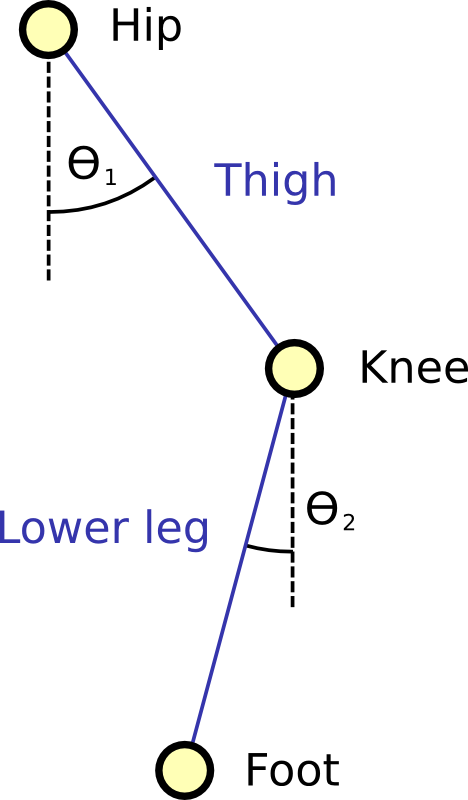
\includegraphics[height=6cm]{model1.png}}
	\qquad
	\subfloat[Front view]{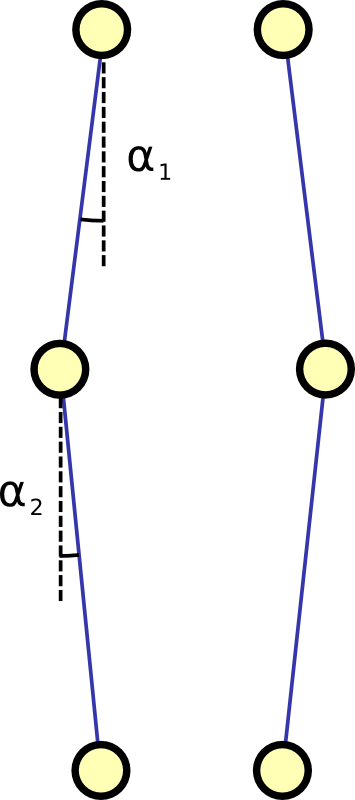
\includegraphics[height=6cm]{model2.png}}
	\caption{Our model for the human leg.}
	\label{ModelImages}
\end{figure}
